\chapter{Atomic Magnetometry\label{ch:magnetometry}}


 In the following chapter, there will be given an introduction into the quantum mechanical
structure and interactions of a Rb atom with special focus on the hyperfine structure and the Zeeman splitting of the energy levels in an external magnetic field. In the second section of this chapter, the principle of atom-light interactions including optical pumping
will be explained. After introducing basic concepts of alkali atom quantum mechanics, the phenomenology of nonlinear magneto-optical rotation (NMOR) will be discussed, which is the basis for the operation of an atomic magnetometer as it will be used for the nEDM setup

A possible outline of this Chapter.
\begin{itemize}
\item Atomic structure of Rb

Alkali-metal atoms have single electron in their outer shell. For this reason they are often used for optical pumping. Alkali-metal atoms have a nuclear spin.
 Because of the nuclear spin the energy level of these alkali atom becomes complicated.
  \begin{itemize}
  \item g.s.and e.s ($L$, $S$)
  
  
  \item fine structure ($J$)
  
  \item hyperfine structure ($F$)
  
  
  \item Selection rules ($\Delta l$, $\Delta J$, $\Delta F$, $\Delta
    M_l$), D1 and D2 lines of Rb
    
  
  \item Doppler broadening and Rb absorption spectrum (of D1 line)
  \end{itemize}
\item Linear and nonlinear magneto-optical rotation (mostly from
  Budker, Orlando, Yaschuk Am J Phys)
  \begin{itemize}
  \item Hypothetical transition and linear magneto-optical rotation
  
 In the presence of an axial magnetic field, when a linearly polarized light passes through an atomic medium the plane of polarization rotates. This kind of effect is known as the Faraday effect. Afterwards an resonant enhancement of the Faraday rotation has been discovered by D. Macaluso and O.M Corbino in 1898 which is known as nonlinear magneto-optical rotation (NMOR) or nonlinear Faraday rotation \cite{budker2013optical}. Consider an example system of $ F=~1$ to $F'=~0$ transition (Fig~\ref{fig:Zeemansplitting}).  Linearly polarized light can decompose into two counter-rotating circularly polarized components $\sigma^\pm$. The transferable angular momentum is +1 for left circular polarization, -1 for right circular polarization. 
 
 In the absence of a magnetic field, the $M=\pm 1$ sublevels are
degenerate and the optical resonance frequencies for  the two circular
polarizations coincide. 
 In the presence of magnetic field the Zeeman sublevels $M=\pm 1$ shift in energy  by an amount $g\mu B/\hbar$ where g is the Lande factor and $\mu$~is the Bohr magneton. This Zeeman splitting therefore leads to a difference between the  resonance frequencies for for $\sigma^+$ and
$\sigma^-$ light. The left circularly polarized light experiences refractive index $n_+$ and the refractive index for right circularly polarized light is $n_-$. In this case, optical rotation arises due to the difference in the refractive index 
\begin{equation}
\label{eq:emc}
\phi = \pi(n_+-n_{-})\frac{l}{\lambda} \\
\end{equation}
where l is the length of the medium traversed and $\lambda$ is the wavelength of light. The difference between $n_+$ and $n_-$ is shown in  Fig.\ref{fig:Faraday} . On resonance, the rotation is related to the Zeeman shift in the $M=\pm 1$ sub levels. For light with spectral
width of the absorption line much smaller than the transition width, and for zero
frequency detuning from the resonance, the optical rotation can be estimated as
\begin{equation}
\phi \approx \frac{(2g\mu B)/ \hbar\tau)}{(1+((2g\mu B)/(\hbar\tau))^2 )}\frac{l}{l_0}
\end{equation}
where $2g\mu/\hbar$ is correlated to Zeeman splitting, $\tau$ is the doppler width of the
absorption line (of order GHz), and $l_0$ is the absorption length in the medium. 
\begin{figure}[h]
\centering
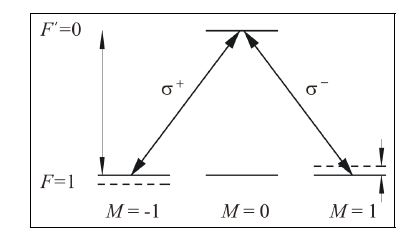
\includegraphics[width=0.75\linewidth]{figures/optical_rotation}
\caption{Illustrative example of F = 1 to $F' = 0$ atomic transition with Zeeman
splitting in the presence of a magnetic field. Image\cite{Budker2002JU2}\label{fig:Zeemansplitting}}
\end{figure}
\begin{figure}[h]
\centering
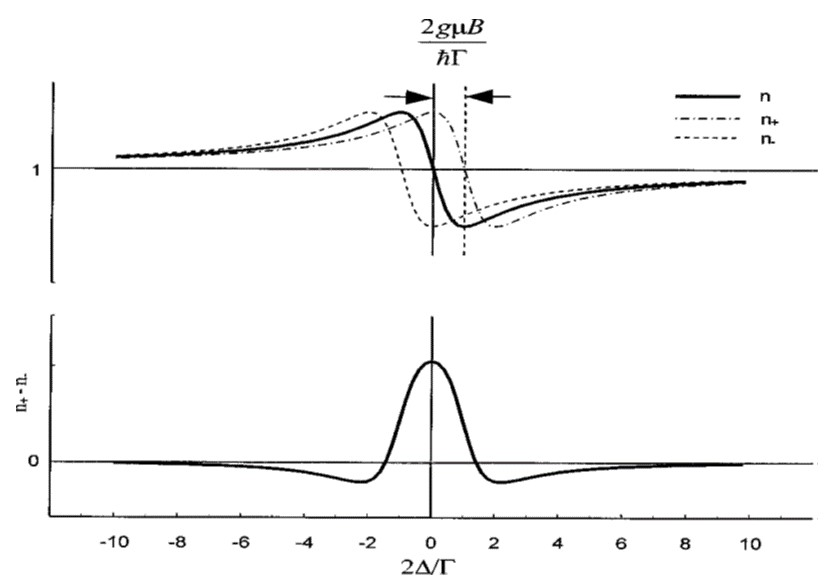
\includegraphics[width=0.65\linewidth]{figures/farday.jpg}
\caption{The dependence of the refractive index on light frequency detuning
D in the absence (n) and in the presence ($n_\pm$) of a magnetic field. Shown is
the case of $2g\mu B=\hbar\tau$ and a Lorentzian model for line broadening. The
lower curve shows the difference in refractive index for the two circular
polarization components. This is the characteristic spectral profile of Macaluso–Corbino opticalrotation. Image\cite{bib:NMOR1998}\label{fig:Faraday}}
\end{figure}
  \item Nonlinear effects in atomic gases: hole-burning and coherent
    population trapping
    

In NMOR, the optical properties of the medium are modified by the laser light, resulting in nonlinear effects such as hole-burning and the creation of a coherent dark state.     
Hole burning is the  nonlinear
effect leading to enhanced Faraday rotation. Spectral holes, or Bennett-structures, are dips in the velocity distribution of a group of atoms produced by pump laser beam. The Faraday rotation produced by atoms with such velocity distribution can be thought of as rotation produced by the Doppler distributed atoms without the hole minus the rotation that would have been produced by the pumped out atoms.

Optical pumping is a process by which light modifies the quantum state of the medium it is transmitting through. Coherent population trapping can be described as the pumping of the atomic system in a particular state, the coherent superposition of the atomic states, which is a nonabsorbing state. The exciting radiation creates an atomic coherence, such that the atom's evolution is prepared exactly out of phase with the incoming radiation and no absorption takes place. In the presence of a magnetic field, the atomic alignment
axis created by the coherent population trapping precesses
around the direction of the field with the Larmor frequency.
  \item Nonlinear magneto-optical rotation; also show result from
    Budker PRL 1998.
  \end{itemize}
\item Magnetometry using NMOR


  \begin{itemize}
    \item Near zero field.
    \item Nonzero field.
      \begin{itemize}
      \item FM NMOR 
      
     
      \item AM NMOR
       

      
      \item Michi's thesis

 
      \end{itemize}
    \item Sensitivity to tilted fields
    
    
    \item Vector magnetometer
    
    
  \end{itemize}
\item Reminder of what we do, leading into next chapter
\end{itemize}


\section{Atomic structure of Rb }
\label{sec:Rb structure} 
The ground state structure of the Rb atom is n = 5, L =0~(s-state) and j = 1/2, i.e, $5^2S_{1/2}$. The lowest excited states (L~=1) are the 5p states. According to quantum theory of angular momentum these 5p states have total electron angular momentum J = L + S where L is the orbital angular momentum and S is the electron spin angular momentum. Fine structure splitting occurs due to spin orbit coupling.  The lowest excited states 5P (L~=1, S=1/2) split into  $5^2P_{1/2}$ and $5^2P_{3/2}$  due to the fine structure splitting. The hyperfine structure is a result of the coupling between J and the total nuclear angular momentum I. The total atomic angular momentum F is then given by F~=~J~+I  and the magnitude of F must lie in the range
$J - I \leq F \leq J + I$. For the ground state of~$^{85}{Rb}$, J = 1/2 and I = 3/2, so F = 1 or F = 2. And  for the excited state $5^2P_{1/2}$ ~  which has nuclear angular momentum I = 3/2 and J = 1/2  the allowed values of F are  1 ~and~ 2. The atomic energy levels are shifted according to the value of F. In quantum mechanics, a set of rules tell us the allowed transition between states which are known as selection rules. The rules are that the total orbital angular momentum change should be $\Delta L= \pm 1$ and the change in magnetic quantum number should be $\Delta M_L= 0,\pm 1$. According to selection rules the transitions from the state L=0 to L=1 are possible. Transmission corresponding to the energy difference between the ~$5^2S_{1/2}$~ and~ $5^2P_{1/2}$ levels of rubidium is termed the D1 line; its wavelength is roughly 795 nm\cite{doe:website}.  The ~$5^2P_{3/2}$~state is separated from the ~$5^2S_{1/2}$~ state by an energy corresponding to 780 nm wavelength, it is called the D2 line. Our Rb atomic magnetometer is based on exciting the D1-line transition by optical pumping.  Linearly polarized laser beam is used to induce transitions of electrons from one energy level to another via optical pumping. In this case, the laser beam is tuned to the transition frequency and of sufficient power to perturb the equilibrium distribution of the ground state energy levels. The gyromagnetic ratio of ${85}^Rb$ is 4.667415~Hz/nT~\cite{bib:rb-gyro-reference}.

\section{Rb magnetometry based on NMOR}

A scalar magnetometer requires coherent precession of the spin ensemble, so a resonant excitation must be applied in order to force some large fraction of the atoms to precess together with a common phase. Otherwise the phase of individual atoms is random, and the total transverse spin of the ensemble averages to zero . The sensitivity of NMOR based atomic magnetometer depends on the lifetime of the polarization state. So in this case, it is important to use ground-state polarization since ground-state polarization has a longer lifetime than the excited states. The working principle of a Rb magnetometer can be described as three step process
\begin{itemize}
\item
Resonant light polarizes Rb atoms via optical pumping. Magnetic
moments of the atoms are oriented with respect to the axis of
alignment
\end{itemize}
\begin{itemize}
\item Aligned magnetic dipole moments experience a torque and precess around the axis of the field at the Larmor frequency and medium becomes birefringent
\end{itemize}
\begin{itemize}
\item A linearly polarized probe beam propagating parallel to the
pump beam is passed through the alkali vapor, the plane of polarization of the probe beam
rotates by an angle proportional to the spin component along that direction, and we detect
this rotation in order to observe the spin behavior. optical polarization rotation of a probe beam is used to measure magnetic field
\end{itemize}
\begin{figure}[h]
\centering
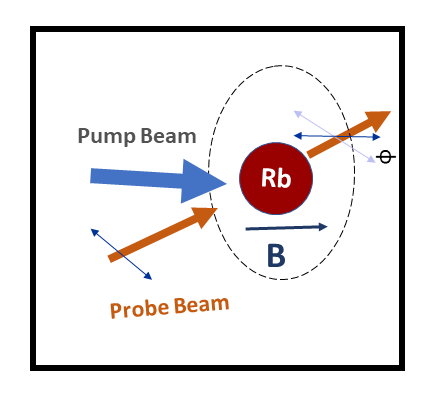
\includegraphics[width=0.55\linewidth]{figures/optical_pumping}
\caption{The schematic diagram of the optical magnetometry technique.
  A linearly polarized pump beam is sent through the vapor cell
  containing natural Rubidium placed in a homogeneous magnetic field
  B.  The polarization rotation of a linearly polarized probe beam is
  used to measure magnetic field,\label{Rb magnetometry}}
\end{figure}

\section{Magnetometry using NMOR\label{sec:magnetometry literature review}}

nonlinear magneto-optical rotation (NMOR), is a promising technique for a new generation of ultrasensitive atomic magnetometers. For magnetic fields directed along the light propagation direction, resonances in NMOR appear when linearly polarized light is frequency or amplitude modulated at twice the Larmor frequency. Because the frequency of these resonances depends on the magnitude but not the direction of the field, they are useful for scalar magnetometry.

 The frequency modulated (FM) NMOR technique is useful for increasing the dynamic range of NMOR-based magnetometers.  It is possible to achieve the  sensitivity of the device in the range of  $10^{−11} $ G/pHz (comparable or superior, e.g., to the most sensitive superconducting quantum interference (SQUID) sensors)\cite{bib:FMNMOR}.

 Studies have been reported by  Pustelny et al.\cite{bib:AMNMOR,bib:amNMOR} on all-optical magnetometric technique based on nonlinear magneto-optical rotation with amplitude-modulated light. To extent the magnetometer sensitivity to magnetic fields where Larmor
precession is much faster than the ground state relaxation rate, it is
necessary to synchronize the optical pumping rate with Larmor
precession which can be achieved by modulating the light
\cite{doi:10.1063/1.3225917}. In AM NMOR, the atoms need to be pumped repeatedly. When this modulation frequency is the same as the harmonic
frequency of the atoms we observe NMOR signal. The method enables sensitive magnetic-field measurements in a broad dynamic range. The sensitivity of  $4.3\times10^{-9}$ G/$\sqrt{\text{Hz}}$ at 10 mG and the magnetic field tracking in a range of 40 mG has been achieved. 

An all-optical magnetometer is also capable of measuring the direction of a magnetic field along with field magnitude \cite{bib:vectormagnetometer}.  This study has been conducted using nonlinear magneto-optical rotation in cesium vapor.  Vector capability is added by effective modulation of the field along orthogonal axes and subsequent demodulation of the magnetic-resonance frequency.  The sensor exhibits a demonstrated rms noise floor of   65 fT/$\sqrt {Hz}$ in measurement of the field magnitude and $ 0.5$  mrad/$\sqrt {Hz}$ in the field direction.  Applications for this all-optical vector magnetometer would include magnetically sensitive fundamental physics experiments, such as the search for a permanent electric dipole moment of the neutron. 

Pustelny et al. \cite{PhysRevA.74.063420}  showed that when the magnetic field is along the light propagation direction, the main resonance occurs at $\Omega_m = 2\Omega_L$. This resonance appear because of the symmetry of the optically pumped state.  In this case, the amplitude of resonance signal decreases with increasing tilt angle . However, If we tilt the magnetic field direction towards the light polarization axis a new resonance appears at $\Omega_L$ along with the main resonance at $2\Omega_L$ if linearly polarized light is used. The amplitude of the new resonance signal at $\Omega_L$  increases as the angle between B and the light propagation direction increases while main resonance amplitude at $2\Omega_L$  decrease with increasing tilt angle. However,when the tilt angle is larger than some certain angle the resonance amplitude measured at $\Omega_L$ also start to decrease and reaches zero when the magnetic field is directed along the y axis.   It could be possible to evaluate the magnitude of the magnetic field from the ratio of the resonance amplitudes at $\Omega_L$ and $2\Omega_L$. The ratio of the resonance amplitudes at $\Omega_L$ and $2\Omega_L$ can be used to
evaluate the magnitude of the B-field at the measuring point.

 To achieve further sensitivity another way of receiving a signal from the magnetometer
has been studied \cite{mythesis}. In this study an all optical magnetometer has been operated in Free Induction Decay (FID) mode where the Cs atoms have to be excited
once and afterwards the decaying processes (damped oscillation) of the coherence state is
observed (similar to NMR). The sensitivity depends on the $T_2$ time, which is the decay time
of the macroscopic polarization moment.

In self-oscillation mode\cite{PhysRevA.62.043403}, the output signal
of photodiode is fed back to AOM for amplitude modulation. In this
case the output signal of polarimeter is modified to act as a square
wave which drives the AOM directly. After setting the phase and gain
of the feedback system properly, the system start to oscillates
spontaneously at the Larmor frequency. In order to measure the
oscillation frequency a frequency counter can be used in this mode. An
online tracking of the oscillating signal is also possible.

Advantages: Being a quite fast process and having a high bandwidth are
the main features of this self-oscillation scan. In order to get rapid
update of the magnetic field the magnetometer can be operated in this
mode.

%Disadvantages: Since feedback loop self-oscillate in the case of
%constructive interference, it will work only for the signal having a
%phase shift of integer multiple of $2\pi$. This additional phase shift
%might be resulting into slightly off-centered resonance. As a result,
%self-oscillation mode is more susceptible to systematic errors in
%field measurement.
